\textcolor{red}{In this section, we explain information about the test problems and corresponding instances in summarized manner. This includes type, components, and instances for each problem. More detailed problem-specific explanation is available in Section \ref{sec:prob_desc}.}
\subsection{Type of problems}
\begin{table}[H]
	\centering
	\caption{Types of the problems in \texttt{SIPLIB 2.0}}
	\label{table:prob_type}
	\resizebox{\textwidth}{!}{%
		\begin{tabular}{@{}llll@{}}
			\toprule
			Problem		  		  & Description                                                        & Main reference              \\ \midrule
			\texttt{DCAP}         & Dynamic capacity planning with stochastic demand                   & Ahmed and Garcia \cite{journal:AG2004}                          \\
			\texttt{DCLP}		  &	Data center location problem									   & Kim et al. \cite{journal:KYZC2017}								\\	
			\texttt{MPTSPs}       & Multi-path traveling salesman problem with stochastic travel costs & Tadei et al. \cite{journal:TPP2017}                            \\
			\texttt{SIZES}        & Optimal product substitution with stochastic demand                & Jorjani et al. \cite{journal:JSW1999}          \\
			\texttt{SMKP}		  & Stochastic multiple knapsack problem                               & Angulo et al. \cite{journal:AAD2014}                            \\
			\texttt{SSLP}         & Stochastic server location problem                                 & Ntaimo and Sen \cite{journal:NS2005}                           \\
			\texttt{SUCW}         & Wind power stochastic unit commitment				               & Papavasiliou and Oren \cite{journal:PO2013}                       \\ \bottomrule
		\end{tabular}%
	}
\end{table}

\begin{table}[H]
	\centering
	\caption{Instance naming rules}
	\label{table:naming_rule}
	\resizebox{\textwidth}{!}{%
		\begin{tabular}{@{}lll@{}}
			\toprule
			Problem & Instance name                 & Description                                                                    					      \\ \midrule
			\texttt{DCAP}    & \texttt{DCAP\_$R$\_$N$\_$T$\_$\mathcal{S}$}    &   $R$: number of resources, $N$: number of tasks, $T$: number of time periods, $\mathcal{S}$: number of scenarios        \\
			\texttt{DCLP}	 &								&																										\\
			\texttt{MPTSPs}  & \texttt{MPTSPs\_$D$\_$N$\_$\mathcal{S}$} &$D$: node distribution strategy, $N$: number of nodes, $\mathcal{S}$: number of scenarios\\
			\texttt{SIZES}   & \texttt{SIZES\_$\mathcal{S}$}                            & $\mathcal{S}$: number of scenarios   															\\
			\texttt{SMKP}    &   \texttt{SMKP\_$I$\_$\mathcal{S}$}    &   $I$:number of types for item, $\mathcal{S}$: number of scenarios  													 \\
			\texttt{SSLP}    &   \texttt{SSLP\_$I$\_$J$\_$\mathcal{S}$}      &    $I$: number of clients, $J$: number of server locations, $\mathcal{S}$: number of scenarios                 				   \\
			\texttt{SUCW}    & 	\texttt{SUCW\_$D$\_$\mathcal{S}$}    &  $D$: day type, $\mathcal{S}$: number of scenarios                                                 						 \\ \bottomrule
		\end{tabular}%
	}
\end{table}

%\begin{table}[H]
%	\centering
%	\caption{Constraint type legend \cite{MIPLIB}}
%	\label{table:constraint_type}
%	\begin{tabular}{@{}lll@{}}
%		\toprule
%		Type           & Description        & Constraint form                                                                                           \\ \midrule
%		\texttt{AGG} & Aggregation        & $a_i x_i+a_k x_k=b,\ x_i , x_k$ int. or cont., $a_i , a_k , b \in \mathbb{R}$                  \\
%		\texttt{VBD} & Variable bound     & $x_i \le a_k x_k + b$ or $x_i\ge a_k x_k + b$, $x_i, x_k$ int. or cont., $a_k, b\in\mathbb{R}$ \\
%		\texttt{PAR} & Set partition      & $\sum x_i = 1,$ $x_i$ binary                                                                   \\
%		\texttt{PAC} & Set packing        & $\sum x_i \le 1,$ $x_i$ binary                                                                 \\
%		\texttt{COV} & Set cover          & $\sum x_i \ge 1,$ $x_i$ binary                                                                 \\
%		\texttt{CAR} & Cardinality        & $\sum x_i = b,$ $x_i$ binary, $b\in\mathbb{N}$                                                 \\
%		\texttt{EQK} & Equality knapsack  & $\sum a_i x_i = b,$ $x_i$ binary, $a_i , b\in\mathbb{N}$                                       \\
%		\texttt{BIN} & Bin packing        & $\sum a_i x_i  + a_k x_k \le a_k,$ $x_i$ binary, $a_i , a_k\in\mathbb{N}$                      \\
%		\texttt{IVK} & Invariant knapsack & $\sum x_i \le b,$ $x_i$ binary, $b\in\mathbb{N}$                                               \\
%		\texttt{KNA} & Knapsack           & $a_i x_i \le b$, $x_i$ binary, $a_i,b\in\mathbb{N}$                                            \\
%		\texttt{IKN} & Integer knapsack   & $a_i x_i \le b$, $x_i\ge 0$ integer, $a_i,b\in\mathbb{N}$                                      \\
%		\texttt{M01} & Mixed binary       & $\sum a_i x_i + \sum p_j s_j \le$ or $=b$, $x_i$ binary, $s_j$ cont., $a_i, p_j\in\mathbb{R}$  \\
%		\texttt{GEN} & General            & All other constraint types                                                                     \\ \bottomrule
%	\end{tabular}
%\end{table}

\begin{table}[H]
	\centering
	\caption{Components of the problems ($\mathbb{C},\mathbb{B},\mathbb{I}$: continuous, binary, integer variables)}
	\label{table:prob_class}
	\begin{tabular}{@{}lllll@{}}
		\toprule
		& \multicolumn{2}{l}{1st stage}                              				  	& \multicolumn{2}{l}{2nd stage}                             			        \\ \midrule
		Problem 	     & Variable                    & Constraint                   	& Variable                    & Constraint                  				    \\ \midrule
		\texttt{DCAP}    & $\mathbb{C}$, $\mathbb{B}$  & \texttt{VBB}                	& $\mathbb{B}$                & \texttt{PAR}, \texttt{M01} 			    		\\
		\texttt{DCLP}	 &							   &								& $\mathbb{C}$			 	  &													\\				
		\texttt{MPTSPs}  & $\mathbb{C}$, $\mathbb{B}$  & \texttt{PAR}, \texttt{GEN}		& $\mathbb{B}$                & \texttt{GEN}               						\\
		\texttt{SIZES}   & $\mathbb{I}$ 			   & \texttt{VBD}, \texttt{GEN} 	& $\mathbb{B}$, $\mathbb{I}$  & \texttt{IKN}             						\\
		\texttt{SMKP}    & $\mathbb{B}$                & \texttt{KNA}                	& $\mathbb{B}$                & \texttt{KNA}              						\\
		\texttt{SSLP}    & $\mathbb{B}$                & \texttt{IVK}, \texttt{GEN} 	& $\mathbb{C}$, $\mathbb{B}$  & \texttt{GEN}             						\\
		\texttt{SUCW}    & $\emptyset$                 &                              	& $\mathbb{C}$, $\mathbb{B}$  &                             					\\ \bottomrule
	\end{tabular}
\end{table}


\begin{table}[H]
	\centering
	\caption{Number of the components in each problem (for convenience, we skip the cardinality sign $|\cdot|$ for sets, i.e., for any set $S$, $S$ denotes the number of elements $|S|$ in this table)}
	\label{table:num_components}
	\resizebox{\textwidth}{!}{%
		\begin{tabular}{@{}cccccc@{}}
			\toprule
			&               & \multicolumn{4}{c}{Components}                                                                         \\ \cmidrule(l){3-6} 
			&                & \#Continuous   & \#Binary                           & \#Integer            & \#Constraint              \\ \midrule
			\multirow{3}{*}{\texttt{DCAP}}   & 1st stage & $RT$           & $RT$                               & -                    & $RT$                      \\
			& 2nd stage & -              & $\left(1+R\right)NT$               & -                    & $(R+N)T$                  \\ \cmidrule(l){2-6} 
			& Total          & $RT$           & $RT+\left(1+R\right)NT\mathcal{S}$ & -                    & $RT+(R+N)T\mathcal{S}$    \\ \midrule
			\multirow{3}{*}{\texttt{DCLP}}   & 1st stage &                &                                    &                      &                           \\
			& 2nd stage &                &                                    &                      &                           \\ \cmidrule(l){2-6} 
			& Total          &                &                                    &                      &                           \\ \midrule
			\multirow{3}{*}{\texttt{MPTSPs}} & 1st stage & $(N-1)N$          & $(N-1)N$                              & -                    & $N^2+2N-1$                \\
			& 2nd stage & -              & $(N-1)NK$                            & -                    & $(N-1)N$                     \\ \cmidrule(l){2-6} 
			& Total          & $(N-1)N$          & $(N-1)(1+K\mathcal{S})N$              & -                    & $(1+\mathcal{S})N^2+(2-\mathcal{S})N-1$ \\ \midrule
			\multirow{3}{*}{\texttt{SIZES}}  & 1st stage & -              & $NT$                               & $NT$                 & $(1+N)T$                  \\
			& 2nd stage & -              & -                                  & $N^2 T$              & $2NT$                     \\ \cmidrule(l){2-6} 
			& Total          & -              & $NT$                               & $(1+N\mathcal{S})NT$ & $(1+N+2N\mathcal{S})T$    \\ \midrule
			\multirow{3}{*}{\texttt{SMKP}}   & 1st stage & -              & $2I$                               & -                    & $J$                       \\
			& 2nd stage & -              & $I$                                & -                    & $K$                       \\ \cmidrule(l){2-6} 
			& Total          & -              & $(2+\mathcal{S})I$                 & -                    & $J+K\mathcal{S}$          \\ \midrule
			\multirow{3}{*}{\texttt{SSLP}}   & 1st stage & -              & $J$                                & -                    & $1$                       \\
			& 2nd stage & $J$            & $IJ$                               & -                    & $I+J$                     \\ \cmidrule(l){2-6} 
			& Total          & $J\mathcal{S}$ & $(1+I\mathcal{S})J$                & -                    & $1+(I+J)\mathcal{S}$      \\ \midrule
			\multirow{3}{*}{\texttt{SUCW}}   & 1st stage &                &                                    &                      &                           \\
			& 2nd stage &                &                                    &                      &                           \\ \cmidrule(l){2-6} 
			& Total          &                &                                    &                      &                           \\ \bottomrule
		\end{tabular}%
	}
\end{table}


\begin{figure}[H]

	\label{fig:sparsity}
\end{figure}

\begin{figure}[H]
	\centering
	\subfloat[][DCAP_3_3_3_3]
	{
		\centering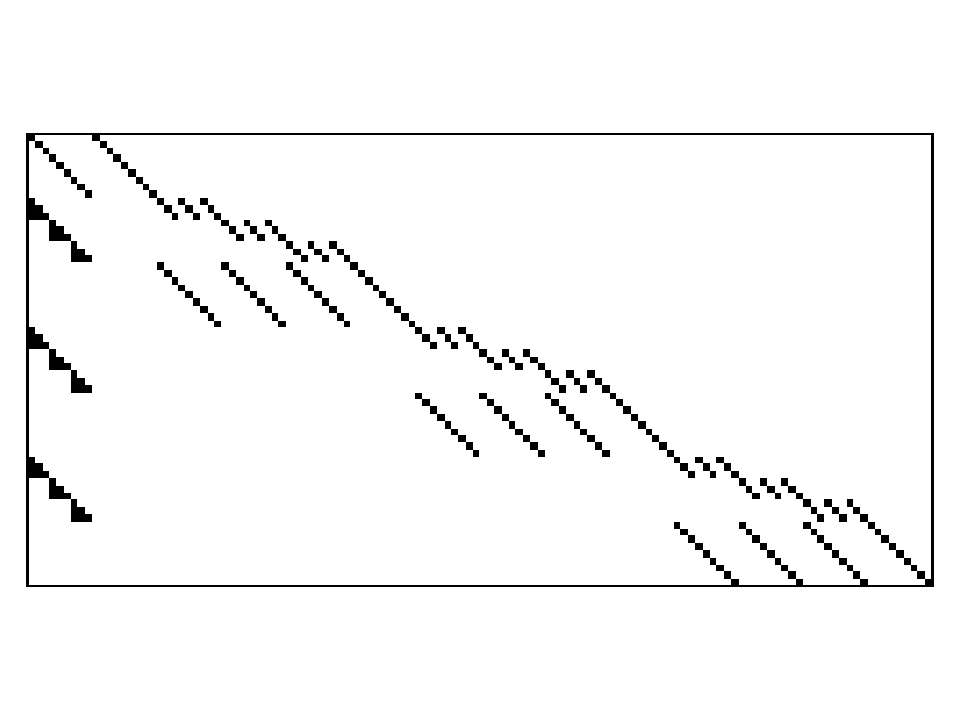
\includegraphics[width=0.48\linewidth]{DCAP_3_3_3_3}
		\label{fig:sparsity_dcap}
	}
	~
	\subfloat[][MPTSPs_D0_3_3]
	{
		\centering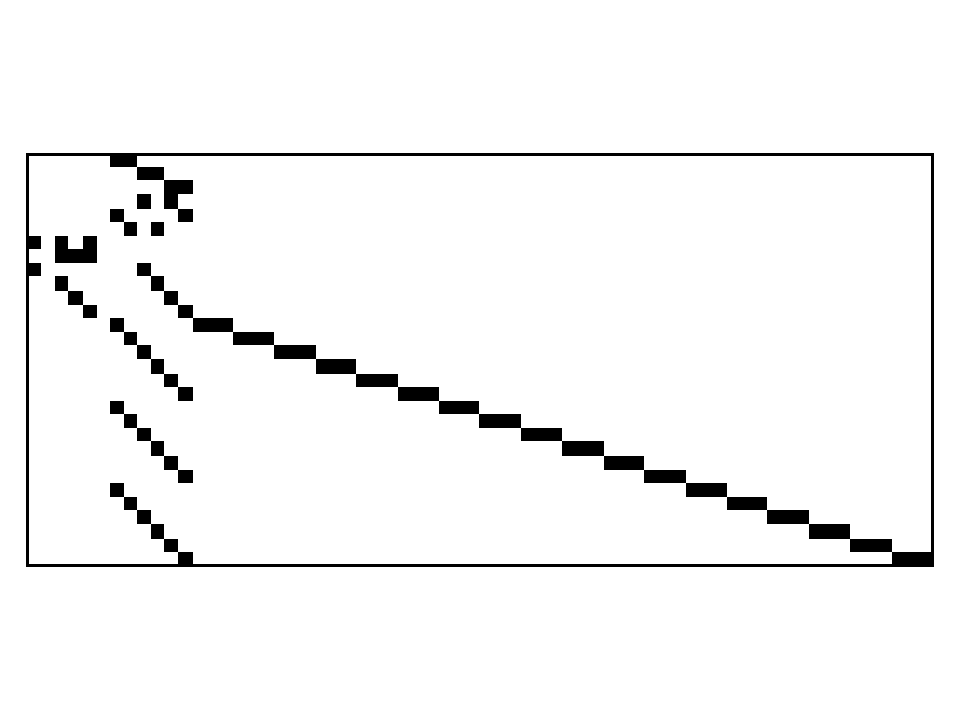
\includegraphics[width=0.48\linewidth]{MPTSPs_D0_3_3}
		\label{fig:sparsity_mptsps}
	}
	
	
	\subfloat[][SIZES_3]
	{
		\centering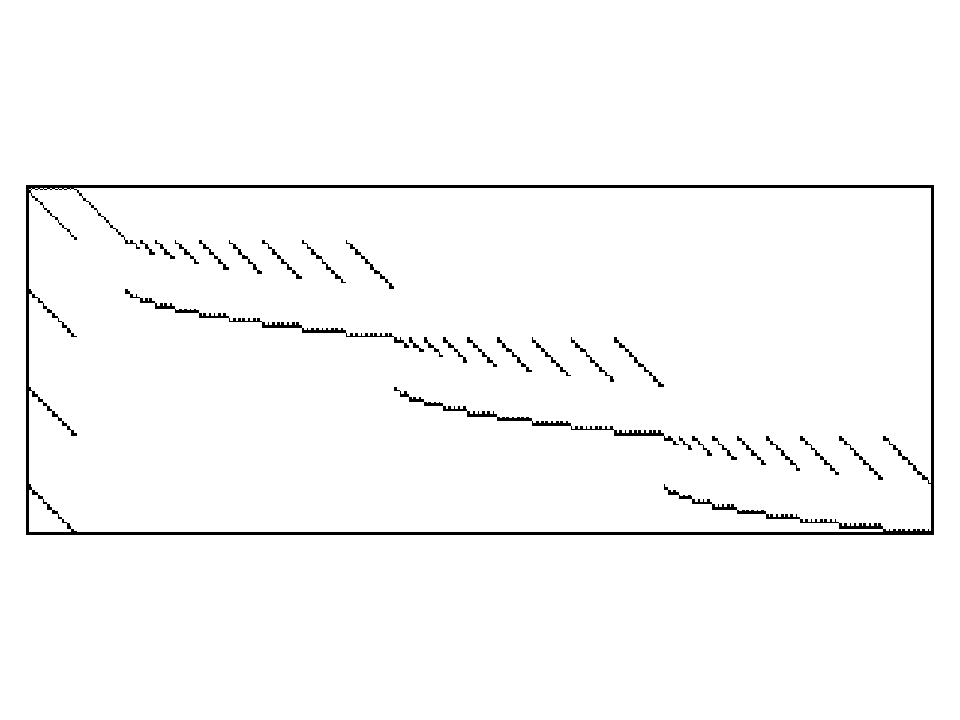
\includegraphics[width=0.48\linewidth]{SIZES_3}
		\label{fig:sparsity_sizes}
	}
	~
	\subfloat[][SMKP_3_3]
	{
		\centering\includegraphics[width=0.48\linewidth]{SMKP_3_3}
		\label{fig:sparsity_smkp}
	}
	\caption{Sparsity pattern for each problem with the number of scenarios 3}
	\label{fig:sparsity}
\end{figure}
\subsection{Instance catalog}


